\chapter{Metodologia}
\label{c:metodologia}
\section{Recollida de documenació i informació}
Un cop detectat que als estudiants del científic els falta material específic per preparar l'examen de MACs a les PAU, vaig fer una recerca de la informació que hi havia de material específic per a la preparació d'aquest examen a través d'internet i llibres. Només vaig trobar material general en què expliquen molta teoria. Llavors, vaig decidir fer una guia on explicar tots els temes no tractats a les MAT II i que entren a l'examen de MACs II. Les diferències més grans que hi ha de temari són de probabilitat i estadística. Dintre de la probabilitat hi ha: la distribució normal i l'aproximació de la binomial per la normal. D'estadística hi ha: la introducció al mostreig estadístic, l'estimació puntual de la mitjana, la proporció i la desviació típica, i intervals de confiança basats en la distribució normal. Explico cada tema i com afrontar-los a l'examen, per a preparar als alumnes per a assolir la màxima nota a l'examen. Em centro molt més en la part pràctica d'exercicis i no tant en la part teòrica, ja que la teoria es pot trobar en molts llocs, però exercicis concrets com els que hi ha a les PAU són més difícils de trobar, aquí és on el meu treball destaca.

\section{Organització i aprenentatge}
El treball el vaig començar fent una anàlisi exhaustiva dels exàmens de les PAU des del 2000 fins al 2026, buscant exercicis dels temes que havia d'estudiar. Vaig descobrir que, per una reforma curricular, els exercicis rellevants dels temes que tracto només apareixen a partir del 2024. Un cop tenia clar quins temes havia d'explicar per a resoldre aquests exercicis vaig començar a aprendre'm el temari. Vaig estudiar i practicar exercicis amb el llibre de MACs II, amb vídeos per internet i amb explicacions del Fernando Garcia, el meu tutor de TR. Va ser un procés difícil perquè no estava acostumat a estudiar temes sencers pel meu compte, sense cap guia ni planificació, però que val la pena per tot el potencial que té i per la feina i el temps que pot estalviar a altres estudiants.

\section{Redacció i elaboració de la guia}
Quan ja sabia el contingut de cada tema i l'havia practicat amb exercicis, em vaig posar a explicar el tema en la meva guia. L'estructura de l'explicació dels temes és:
\begin{enumerate}
 \item Breu explicació i tan entenedora com sigui possible.
 \item Exercicis resolts, perquè l'estudiant tingui una referència de com fer els exercicis.
 \item Exercicis per practicar, començant per exercicis fàcils i acabant amb exercicis com els de les PAU.
\end{enumerate}



\chapter{Eines}
\label{c:eines}
Cito el treball de recerca del Max Pérez~\cite{TR-MP-2025} en el que explica les eines utilitzades:



``Aquest treball ha requerit combinar diferents eines i metodologies, tant de caràcter tècnic com organitzatiu. En aquest capítol descric el conjunt de recursos utilitzats i la manera com s’han integrat en el procés de recerca, amb l’objectiu de donar una visió clara i transparent del camí seguit.

\section{Entorn de treball}
Per fer aquest treball vaig optar per a treball amb l'ordinador que ens ha proporcionat el Departament d'Ensenyament. Aquest ordinador presenta moltes limitacions pel que fa a instal·lar i configurar programes nous. Per tal de superar aquest inconvenient, vaig optar per treballar dins d'una màquina virtual disponible en els ordinadors del centre. Aquesta màquina virtual està desenvolupada per l'empresa Oracle~\cite{Oracle} i permet instal·lar un sistema operatiu dins d'un altre sistema operatiu. Per tant, la màquina virtual permet que l'usuari configuri l'ordinador com vulgui, podent saltar-se els controls que imposa el Departament d'Ensenyament sense posar en perill la integritat del sistema operatiu principal.

\subsection{Configuració de la màquina virtual}
La màquina virtual de l'ordinador de l'alumnat porta instal·lada Linkat\cite{Linkat}, una distribució de Linux basada en Ubuntu~\cite{Ubuntu}, creada pel Departament d'Ensenyament, que em va permetre:
\begin{itemize}
  \item Accedir a les eines habituals de programació de manera lliure i sense cap cost.
  \item Utilitzar gestors de paquets per instal·lar biblioteques de manera fàcil i segura.
  \item Mantenir un entorn informàticament segur.
  \item Configurar tots els programes i els recursos del sistema d'acord amb les necessitats que he tingut en cada moment.
\end{itemize}

% \subsection{Punts de restauració i seguretat}
% Un dels avantatges principals de treballar amb Linkat és la possibilitat de crear \emph{punts de restauració}:
% \begin{itemize}
%   \item Permeten tornar a un estat estable en pocs minuts si alguna prova falla.
%   \item Faciliten experimentar amb noves biblioteques o actualitzacions sense risc.
%   \item Augmenten la seguretat i la confiança en el procés de desenvolupament.
% \end{itemize}
%
% En conjunt, aquest entorn de treball ha estat clau per avançar amb iteracions ràpides, mantenir la coherència i garantir que el projecte sigui replicable en altres contextos.

\section{Redacció i composició de la memòria}

La memòria s’ha redactat íntegrament amb \LaTeX~\cite{LaTeX}, utilitzant l’editor \textbf{Kile}~\cite{kile}.
Aquesta eina proporciona una interfície amigable per treballar amb documents científics, permet dividir el treball en capítols i seccions, i ofereix eines per compilar ràpidament a PDF.
L’ús de \LaTeX\~ha estat clau per mantenir una presentació professional del text, gestionar remissions (cites internes), cites bibliogràfiques i incloure figures, taules i fórmules sense dificultats.
A més, la redacció en\LaTeX\~facilita la traçabilitat dels canvis, ja que el codi font del document es pot gestionar igual que el codi d’un programa.


\begin{figure}[h!]
  \centering
  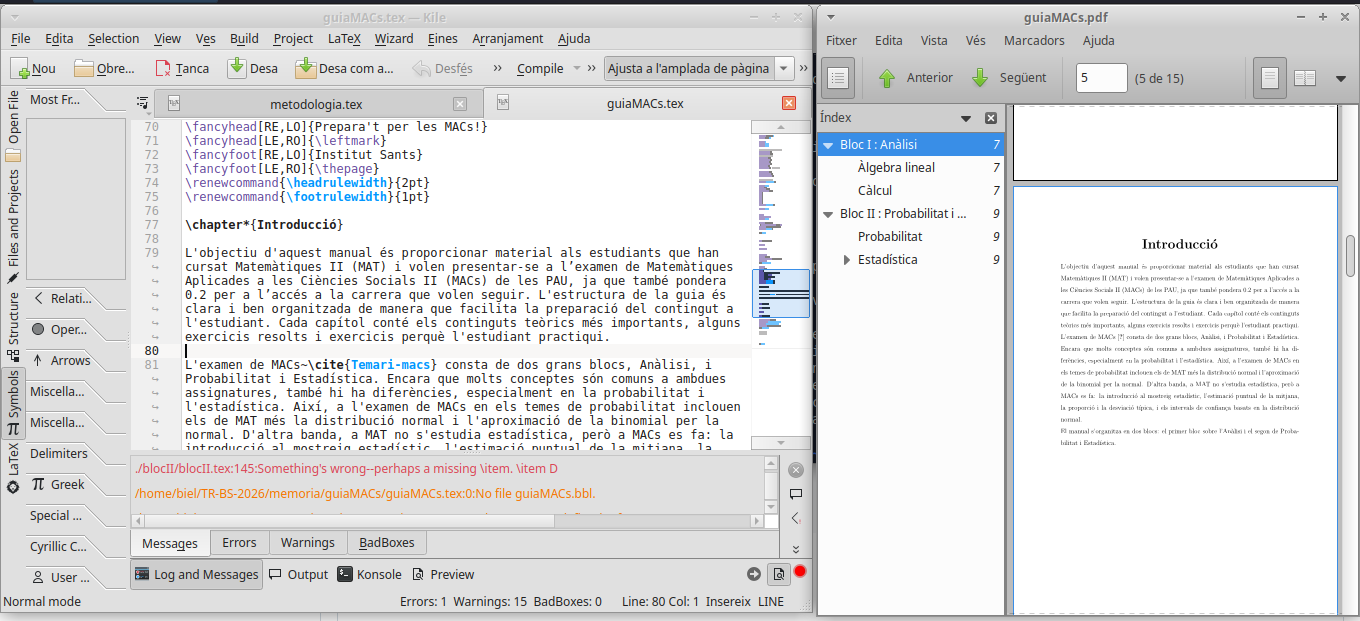
\includegraphics[width=0.85\textwidth]{./figures/memoriaLatex.png}
  \caption{Entorn de redacció de la memòria amb \LaTeX\ i l’editor Kile.}
  \label{fig:memoriaLatex}
\end{figure}

Per tal de mantenir la memòria ordenada i modular, vaig dividir el document en diversos fitxers \texttt{.tex}, un per a cada capítol.
Aquesta estructura facilita la navegació i la revisió, ja que puc editar seccions concretes sense afectar la resta del document.
També vaig utilitzar \texttt{BibTeX} per gestionar la bibliografia, cosa que em permet afegir referències de manera centralitzada i assegurar que totes les cites segueixen un format coherent.

A més, vaig incorporar diversos paquets de \LaTeX\ per millorar la presentació del document: \texttt{graphicx} per a la inclusió de figures, \texttt{float} per controlar la posició dels elements visuals, i \texttt{hyperref} per generar enllaços dins del PDF.
Aquest conjunt d’eines ha fet possible una composició clara, estructurada i visualment atractiva, que reforça el caràcter acadèmic del treball.

\section{Gestió de versions i col·laboració}



Per controlar l’evolució del treball i assegurar la seguretat de la informació, he utilitzat \textbf{GitHub}~\cite{github}, com a plataforma de control de versions basada en Git~\cite{git}. Cada canvi important tant en el codi com en la memòria s’ha enregistrat mitjançant \textit{commit}s, que permeten documentar el progrés i tornar a versions anteriors en cas de necessitat. Aquesta pràctica ha resultat especialment útil quan he rebut comentaris del tutor: he pogut obrir noves branques per provar modificacions i, un cop validades, fusionar-les al projecte principal.

GitHub també ha servit com a espai d’emmagatzematge remot, accessible en qualsevol moment i des de qualsevol dispositiu.
Cada funcionalitat (obtenció de dades, càlcul de distàncies, detecció de transbords, exportació CSV) s'ha implementat en una branca independent i posteriorment fusionada a la branca principal.

El meu treball de recerca s'ha desenvolupat completament al repositori (\texttt{main}) del meu projecte de GitHub TR-BS-2026~\cite{TR-BR-2026}.
Cada \textit{commit} representava un pas endavant en el projecte, i l’historial mostra de manera clara l’evolució del codi i de la memòria.



Treballar d’aquesta manera té avantatges i inconvenients.
Com a punt positiu, el procés és més àgil i directe: qualsevol canvi queda immediatament integrat al projecte principal.
D’altra banda, també implica més responsabilitat, ja que un error en un \textit{commit} afecta directament la versió principal.
Per minimitzar aquest risc, vaig procurar que cada \textit{commit} fos petit i descriptiu, de manera que fos fàcil identificar i revertir un canvi si calia.

A més, GitHub ha funcionat com a còpia de seguretat remota.
En qualsevol moment podia clonar el repositori en un altre ordinador i continuar treballant sense perdre res.
Aquesta característica m’ha donat tranquil·litat i ha assegurat que el projecte fos accessible i recuperable en tot moment.

Cal fer notar que aquest recurs ha dotat el treball de recerca de traçabilitat, de llibertat i facilita la transferència de coneixement, que eren alguns dels objectius del treball.''
